\section{Background}
\label{sec:background}

\gls{nso} foundations can be rooted back to three enabling technologies, namely Cloud Computing, SDN, and NFV. This section provides a brief background on these topics and their relationships to NSO, in addition to a short historical review of the term ``orchestration''.

\subsection{Cloud Computing}
Cloud computing is a model for providing resource virtualization (e.g., networks, servers, storage, and services) with high flexibility, cost efficiency, and centralized management~\cite{Le2016SurveyNetworks}. The cloud computing service models are generally categorized in \gls{iaas}, \gls{paas}, and \gls{saas} which offer, respectively,  virtual resources (compute, storage, and network), software and development platforms (provided by the cloud infrastructure), and Internet-based applications (hosted on the cloud)~\cite{bele2018empirical}.

In a cloud environment, the notion of orchestration has also been used for integrating basic services~\cite{Vouk2008CloudImplementations}. Orchestration in the cloud involves dynamically deploying, managing and maintaining resource and services across multiple heterogeneous cloud platforms in order to meet the needs of clients. 

\subsection{Software Defined Networking (SDN)}
\gls{sdn}~\cite{surveySDN} is an evolving networking paradigm that attempts to resolve the strongly vertical integration of current network environments. To this end, \gls{sdn} proposals decouple the control plane (i.e., control logic) from the data plane (i.e., data forwarding equipment). With this new architecture, routers and switches become simple forwarding network elements whose control logic is provided by a logically centralized external entity called \gls{sdn} controller or \gls{nos}.

In multi-domain scenarios, there are different \gls{sdn} controllers deployed to manage specific segments of a network (e.g., fronthaul, backhaul, and core). \gls{sdn} implements some level of resource orchestration in order to coordinate control plane actions with multiple \gls{sdn} controllers. By recognizing the needs of higher-level  orchestrator(s), \gls{sdn} controllers can be programmed to monitor the network and make automated (real time) decisions in case of security problems, faulty devices, traffic congestion, among others~\cite{SDXCentral2015WhatSDNOrc}. 

\subsection{Network Function Virtualization (NFV)}
\label{subsec:nfv}

According to \gls{etsi} \gls{isg} \gls{nfv} \cite{ETSIIndustrySpecificationGroupISGNFV2014NetworkNFV},  \acrlong{nfv} is responsible for separating network functions from the hardware and offering them through virtualized services, decomposed into \glspl{vnf}, on general purpose servers. With the virtualization of the network functions, \gls{nfv} promises more flexible and faster network function deployment, as well as dynamic scaling of the \glspl{vnf} towards providing finer settings. In \gls{nfv} environment, new services do not require new hardware infrastructure, but simply the software installation, i.e., to create \glspl{vnf}.

\glspl{vnf} can be connected or combined as building blocks to offer a full-scale network communication service. This connection is known as service chain. Within the scope of the \gls{isg} \gls{nfv} \cite{ETSIIndustrySpecificationGroupISGNFV2014NetworkNFV}, service chain is defined as a graph of logical links connecting \glspl{nf} towards describing traffic flow between these network functions. This is equivalent to the \gls{sfc}~\cite{Halpern2015} defined by Service Function Chaining Working Group (IETF SFC WG) of the \gls{ietf}.  
An end-to-end network service may cover one or more \gls{nffg} which interconnect \glspl{nf} and end points.  Figure~\ref{nffg} describes two examples of end-to-end network services. The first (green line) is composed of \gls{vcpe} and \gls{vfw} \glspl{vnf} and two endpoints (A1 and A2). The second (red line) is composed of \gls{vcpe} and \gls{vdpi} \glspl{vnf} and two endpoints (B1 and B2). In the examples, a single VNF can be part of one or more network services. It emphasizes the multi-tenant aspect of \gls{nfv}.

\gls{etsi} has developed a reference architectural framework and specifications in support of NFV management and orchestration. The framework covers orchestration and lifecycle management of physical and virtual resources. According to~\cite{ETSIIndustrySpecificationGroupISGNFV2013NetworkFramework}, ``the framework is described at a functional level and it does not propose any specific implementation." Figure~\ref{mano} shows the \gls{etsi} \gls{nfv}-\acrfull{mano} architectural framework with their main functional blocks~\cite{ETSIIndustrySpecificationGroupISGNFV2014NetworkOptions}:

 \\
 \noindent \textbf{Operation/ Business Support System (OSS/BSS)}: block responsible for operation and business applications that network service providers use to provision and operate their network services. It is not tightly integrated into the \gls{nfv}-\gls{mano} architecture.
 \\
\noindent \textbf{\gls{em}}: component responsible for the network management functions FCAPS (Fault, Configuration, Accounting, Performance, and Security) of a running \gls{vnf}.
\\
\noindent\textbf{\gls{vnf}}: functional block representing the Virtualized Network Function implemented on a physical server. For instance, Router \gls{vnf}, Switch \gls{vnf}, Firewall etc.
\\
\noindent \textbf{\gls{nfvi}}: representing all the hardware (compute, storage, and networking) and software components where \glspl{vnf} are deployed, managed and executed. 
\\
\noindent \textbf{\gls{nfvo}}: it is the primary component, in charge of the orchestration of \gls{nfvi} resources across multiple \glspl{vim} and lifecycle management of network services. 
\\
\noindent\textbf{\gls{vnfm}}: performs configuration and \gls{vnf} lifecycle management (e.g., instantiation, update, query, scaling, termination) on its domain.
\\
\noindent \textbf{\gls{vim}}: block that provides controlling and managing the \gls{nfvi} resources as well the interaction of a \gls{vnf} with hardware resources. For example, OpenStack as cloud platform and OpenDaylight and \gls{onos} as \gls{sdn} controllers.
 

\begin{figure}[t]
  \centering
  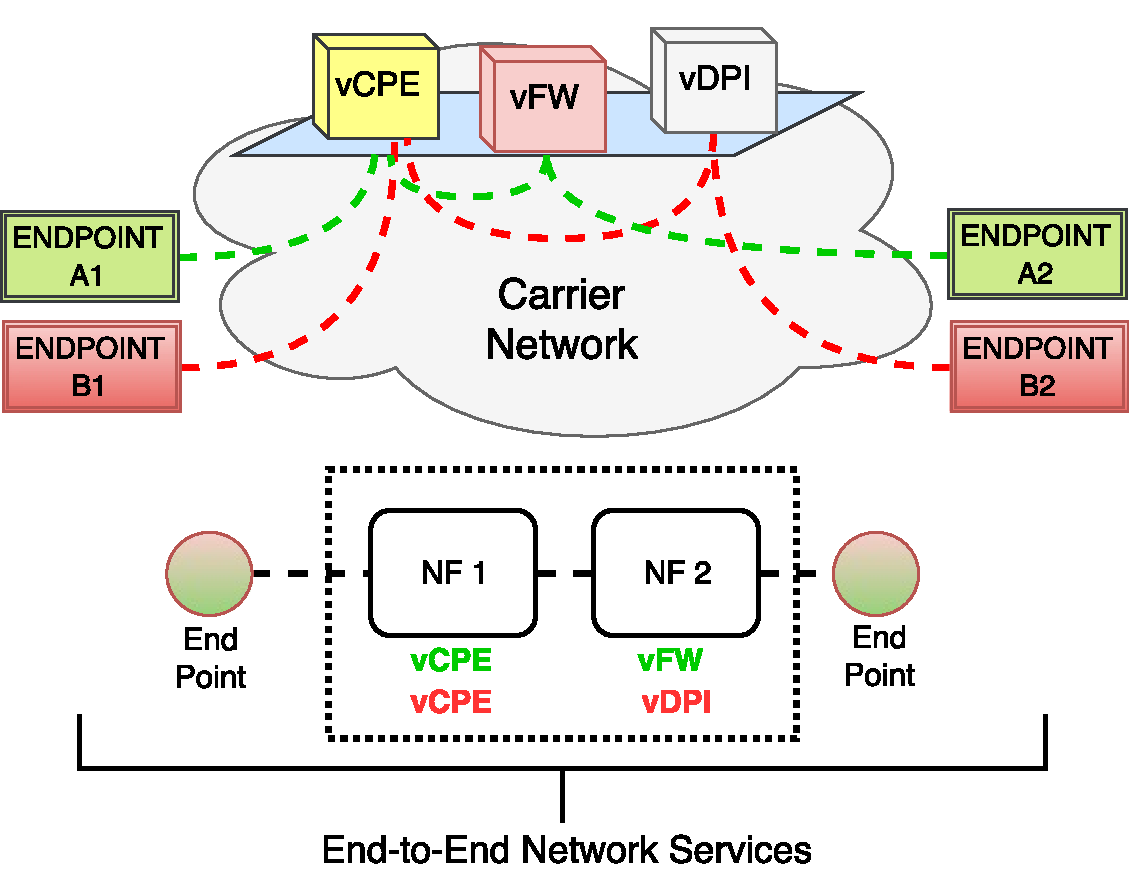
\includegraphics[scale=.46]{Figures/02_Background/fig5.pdf}
    \caption{Example of two end-to-end network services composed of two \glspl{nf} each. NFV enables the reuse of \glspl{vnf}, e.g., \gls{vcpe}.}
    \label{nffg}
\end{figure}

\begin{figure}[t]
  \centering
  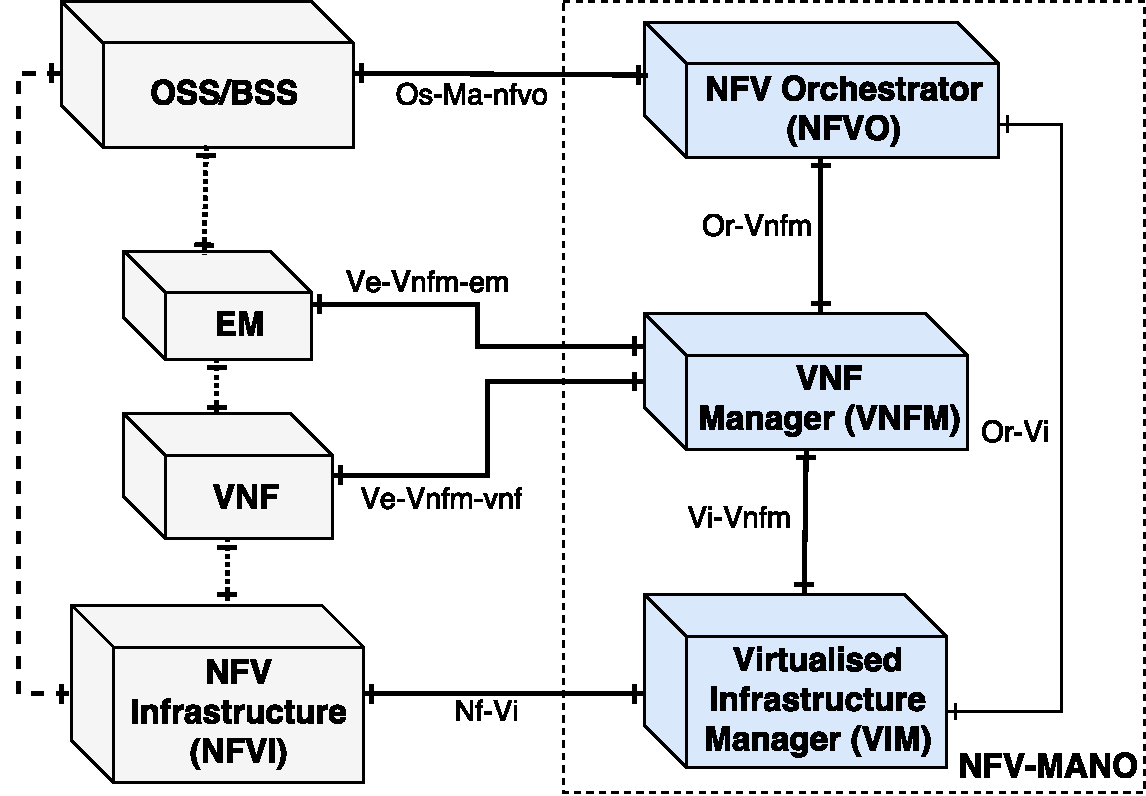
\includegraphics[scale=.45]{Figures/02_Background/fig6.pdf}
    \caption{The \gls{nfvmano} architectural framework. Adapted from \cite{ETSIIndustrySpecificationGroupISGNFV2014NetworkOptions}}
    \label{mano}
\end{figure}

In the \gls{nfv} context, \gls{etsi} \gls{nfvmano} defines the orchestrator with two main functions including \textit{resources orchestration across multiple \glspl{vim}} and \textit{network service orchestration}~\cite{GSNFV-MAN001:2014}. Network service orchestration functions provided by the \gls{nfvo} are listed below:
\begin{itemize}
\item Management of Network Services templates and \gls{vnf} Packages. 
\item Network Service instantiation and management;
\item Management of the instantiation of \glspl{vnfm} and \glspl{vnf} (with support of \glspl{vnfm});
\item Validation and authorization of \gls{nfvi} resource requests from \gls{vnf} managers;
\item Policy management related to affinity, scaling (auto or manual), fault tolerance, performance, and topology.
\end{itemize}

\gls{etsi} \gls{nfvo} functions regarding Resource Orchestration include: (\textit{i})  Orchestration of NFVI resources across multiple \glspl{vim}, (\textit{ii})  \gls{nfvi} resource management including compute, storage and network, and (\textit{iii}) collect usage information of \gls{nfvi} resources. \gls{nfvo} functions defined by \gls{etsi} are limited to the delivery of network services, i.e., without being aware of what type of service has been instantiated.

The \gls{nfvmano} reference architecture is not  specific about \gls{sdn} in its architecture but  assumes that necessary transport infrastructure is already established and ready to be used. However, work at \gls{etsi} identifies use cases and the most common options for using SDN in an NFV architectural framework~\cite{ETSINetworkFramework}. The document also points to  proof of concepts and recommendations towards such integration work.
\cite{nfv-survey18} provides a recent in-depth survey on NFV state of affairs. 

\subsection{Orchestration: Historical Overview}
The academic community and industry generally require some time to define the real meaning, reach and context of the concepts related to new technology trends as is the case with the term \textit{Orchestration}. 
The term orchestration is used in many different areas, such as multimedia, music, \gls{soa}, business processes, Cloud, \gls{sdn}, and, more recently, in \gls{nfv}.

From an end-user perspective, orchestration reminds a symphony orchestra where a set of instruments play together according to an arrangement. The music is arranged and split into small parts, after assigns to different musical instruments. When, who, and what will be played, as well as the conducting are essential parts towards achieving the desired effect. In next paragraphs, we identified the first works that use the term orchestration in other areas. 

One of the first works in the \gls{ict} area that cites the term orchestration is \cite{Anderson1983} in 1983. It discusses that an autonomous system will require orchestration of the behavior of the entire system in order to obtain autonomy, interdependence and artificial intelligence. The authors in~\cite{Campbell1992} relate orchestration with the coordination and control of multiple media traffics. It distinguishes orchestration from synchronization and defines an architecture where orchestration acts in different layers. In the same scope, \cite{Robbins1997ImplementationArchitecture} relates the term to multimedia data, where orchestration is associated with multimedia presentation lifecycle management involving the coordination of stages that constitute all orchestration processes. 

The use of orchestration is also widely discussed in the scope of web services. In this context, orchestration and automation are considered separate processes. The work in~\cite{Peltz2003WebChoreography} defines orchestration like an executable process that can interact both internal and external services and must be dynamic, flexible, and adaptable to changes. It emphasizes that orchestration describe how web services can act with each other at the message level, including the business logic and execution order of the activities. 

The authors in~\cite{Grit2006} present the term orchestration in the context of virtual resource management. They define orchestration as a process that involves all the necessary steps to map the application (running on a virtual machine) onto shared underlying infrastructure. 

Orchestration in the cloud environment is well-known and refers to locating, coordinating and selecting resources, including compute, storage and virtual networks to fulfill the desired requirements. The authors in \cite{Galis2009ManagementInternet} provide an overview of networking architecture definition for the \gls{fi} based on the concepts of cloud computing. One of the pillars for the \gls{fi} pointed out by the article is Orchestration. In the envisioned architecture, the orchestration function is to coordinate the integrated behavior and operations to dynamically adapt and optimize resources in response to changing context following business objectives and policies.

In the \gls{sdn} landscape, orchestration refers to an overarching function to manage and automate the network behavior~\cite{5984813}. More recently in 2012~\cite{ETSI2012NetworkAction}, orchestration has been generally related to \gls{nfv} environments mainly through its reference architecture and its \gls{nfv} Orchestrator component (more details in Subsection~\ref{subsec:nfv}).  

Currently, the scope of orchestration has become broader and encompasses automation of the end-to-end network service lifecycle. According to \cite{MEF:Third:2015}, service orchestration refers to the programmatic control of underlying infrastructure including existing networks and enabling technologies, such as SDN and NFV.

From the existing and evolving definitions around orchestration presented, we can derive certain relationships between orchestration, automation, and management. Although the three terms are often lumped together, it is necessary an understanding of the differences between them as they are not the same thing. Automation describes a simple and technical task without the human intervention, for example, launching a web server, stopping a server. Management is responsible for maintaining and healthiness of infrastructure. Its role consists of activities such as alarms for event detection, monitoring, backups of critical systems, upgrades, and license management. Orchestration, in turn, is concerned with the execution of a workflow (processes) in the correct order. It controls the overall workflow process from starting the service until it ends with the objective to optimize and automate the network service deployment. 

Figure~\ref{diff} illustrates the relationship among orchestration, management, and automation through a hierarchy. Orchestration is a high-level plane followed by  the management layer. Automation lies at the lower layer. In our vision, the orchestration layer depends on tasks performed by management. Both management and orchestration are based on the use of automation in the execution of their tasks. Nevertheless, several activities are only performed by a certain function: optimization, for instance, cannot be achieved through simple automation. 

\begin{figure}[t]
    \centering
    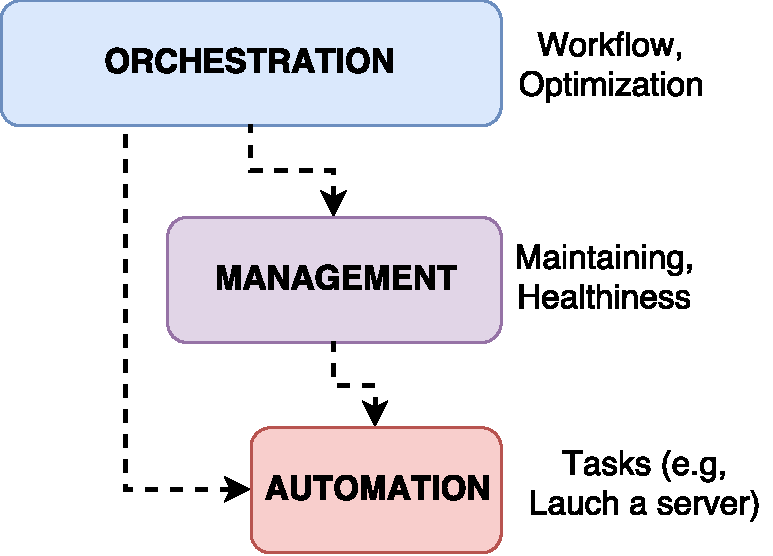
\includegraphics[scale=.45]{Figures/02_Background/fig7.pdf}
      \caption{Relationship among orchestration, management, and automation. Both orchestration and management use automation in their processes.}
      \label{diff}
\end{figure}

Based on all the above-mentioned background, in short, \gls{nso} is in charge of the full network service lifecycle to deliver end-to-end connectivity along additional services. To this end, orchestration is supported by advances in cloud computing, and technologies such as \gls{sdn} and \gls{nfv}, which offer the ability to reconfigure the network quickly as well as programming the forwarding and processing of the traffic. Figure~\ref{nso_rel} shows how \gls{nso}, \gls{nfv}, \gls{sdn}, and Cloud Computing work together.

Each one of these paradigms/technologies has different functions: high level orchestration for \gls{nso}, function programming for \gls{nfv}, networking programming for \gls{sdn},  and resource virtualization for cloud computing. Note that such technologies are complementary in order to provide complete management of the network services lifecycle. Although they have different functions, they share a common feature: \textit{orchestration}. They can work in an integrated pattern to offer advantages such as agility, cost reduction, automation, softwarization, and end-to-end connectivity, to enable novel services and applications such as 5G networks.

\begin{figure}[t]
  \centering
  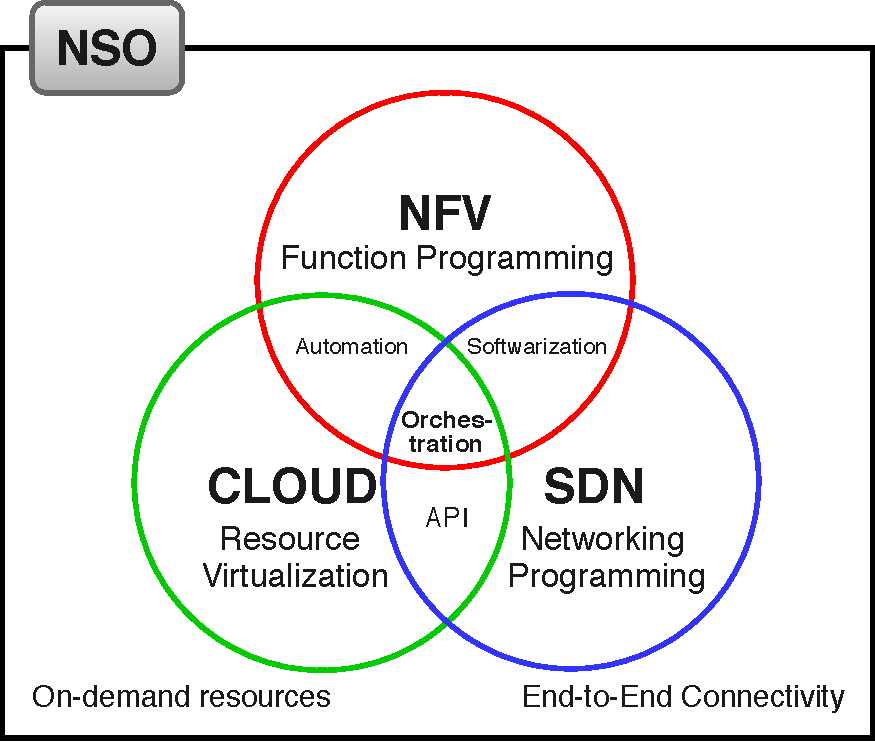
\includegraphics[scale=.58]{Figures/02_Background/fig8.pdf}
    \caption{Illustration of relationships among \gls{nso}, \gls{nfv}, \gls{sdn}, and Cloud.}
    \label{nso_rel}
\end{figure}

Our goal in this subsection was to set the ground and identify the main areas in which the term orchestration is inserted and how it is approached at a high level. An overview of the term usage is illustrated in the timeline of Table~\ref{timeline}. The focus of this survey is to detail the orchestration process in the context of the implementation and operation of network services by operators and service providers.

\begin{table}[!]
\small
\caption{Historical timeline of term orchestration }\vskip -1ex
\label{timeline}
\begin{tabular}{@{\,}r <{\hskip 2pt} !{\foo} >{\raggedright\arraybackslash}p{5cm}}
\addlinespace[3ex]
\toprule
1983 & Autonomous system~\cite{Anderson1983}\\[13.5pt]
1992 & Media Traffic~\cite{Campbell1992}\\[7.5pt]
1997 & Multimedia presentation lifecycle management~\cite{Robbins1997ImplementationArchitecture}\\[1pt]
2003 & Web Service~\cite{Peltz2003WebChoreography}\\[4.5pt]
2006 & Virtual resource management~\cite{Grit2006}\\[4.5pt]
2009 & Cloud computing~\cite{Galis2009ManagementInternet}\\[3pt]
2011 & Software Defining Network~\cite{5984813}\\[1.5pt]
2012 & Network Function Virtualization~\cite{ETSI2012NetworkAction}\\[2pt]
2015 & Lifecycle Service Orchestration~\cite{MEF:Third:2015}\\
\end{tabular}
\end{table}